\documentclass[preprint,proceedings]{rmaa}


%%%
%%% Define any personal macros here
%%% 

% These are some I use in typesetting example code
\newcommand{\bs}{\textbackslash}
\newcommand{\CS}[1]{\texttt{\textbackslash #1}}
% roman subscripts in math
\newcommand{\Sub}[1]{_\mathrm{#1}}
% a command to specify possible linebreak points in an email address 
\newcommand{\D}{\discretionary{}{}{}}

%%%
%%% Article preamble commands (title, authors, abstract, etc.) 
%%% None of these produce any output themselves, they just set things 
%%% up for \maketitle
%%%

% This is only used for making the header for the preprint version
\SetYear{2016}
\SetConfTitle{XV LARIM}

% Please use mixed case here, since this title gets propagated onto
% the web page, ADS entry, etc. 
  \title{The influence of environment on the HI mass functions in cosmological simulations}
  
 \author{Jesus D. Prada-Gonzalez\altaffilmark{1}, Michael G. Jones \altaffilmark{2}, J. E. Forero-Romero\altaffilmark{1} and Martha P. Haynes \altaffilmark{2}}

\altaffiltext{1}{Departamento de F\'isica, Universidad de los Andes,
    Cra 1 18A-10, Bloque Ip, Bogot\'{a}, Colombia.}
    
\altaffiltext{2}{Center for Radiophysics and Space Research,
  Space Sciences Building, Cornell University, Ithaca, NY
  14853, USA.}

  % List of authors used to construct table of contents
  \listofauthors{Jesus Prada, Michael G. Jones, J. E. Forero-Romero and Martha P. Haynes}
  % Each author in Surname, Initials format, used in generating Author
  % Index entries.
  \indexauthor{Prada-Gonzalez, J. D.}
  \indexauthor{Jones, M. G.}
  \indexauthor{Forero-Romero, J. E.}
  \indexauthor{Haynes, M. P.}


% No \abstract or \resumen for poster papers

% Keywords must be from the standard list and in alphabetical order. 
\addkeyword{HI mass funcions}
\addkeyword{Environment}
\addkeyword{Schechter functions}
\addkeyword{Nearest neighbour}
\addkeyword{Cosmic web}


%%%
%%% Beginning of document proper
%%%
\begin{document}
 % Typeset article header
\maketitle 
%%%Resumen en Español%%%
\boldabstract{Usamos la simulaci\'on
  Illustris para medir el efecto del entorno sobre las funciones de masa de
  galaxias. Descubrimos, con dos definiciones de entorno de naturaleza
  distinta, que este afecta el lugar del quiebre de la funci\'on de
  masa, mientras que la pendiente a bajas masas no muestra un cambio
  considerable. Esto muestra un acuerdo con el trabajo de Jones et al.}

%%%Abstract%%%

\boldabstract{We use the Illustris simulation to study the effect of
  environment on mass functions.
  We find that the knee-mass parameter changes in different environment.
  while the low mass slope does not show any clear change.
  These results in agreement with previous results by Jones et al.}\\

We use the Illustris Simulation \citep{Vogelsberger}
to measure the Schechter functions for the stellar mass.
We split the galaxies according to its large scale environment
defined by two different criteria.
We aim at quantifying the differences in the Schecter parameters as a
function of environemtn.

The first environment definition is a computational
adaptation of the fourth nearest neighbour method used 
in an observational study of HI galaxies \citep{Jones}. 
We classify galaxies in four quartiles according to this environment
definition and obtained the mass and Schechter functions for each
one. Figure \ref{fig1} shows our results, the environments are ordered
from top to bottom.


\begin{figure}[h!]
\centering
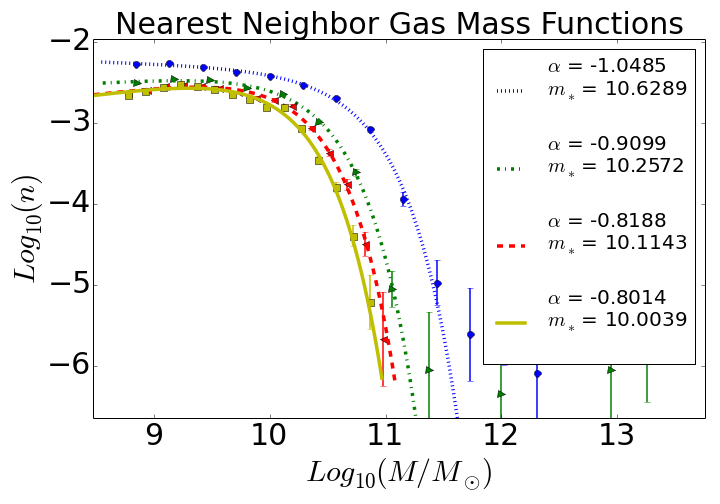
\includegraphics[width=0.5\textwidth]{environment1}
\label{fig1}
\caption{Mass functions with the environment defined from the 4th
  nearest neighbor}
\centering
\end{figure}

The second definition of environment is based 
the Hessian of the gravitational potential \citep{Forero}, or
the Tidal Tensor.
This method classifies the environment according to the number of
eigenvalues of this tensor which are larger than a given threshod. 
The classification is done into voids, filaments, sheets and
clusters. 
Figure \ref{fig2} shows the results for this environment
classification.


\begin{figure}[h!]
\centering
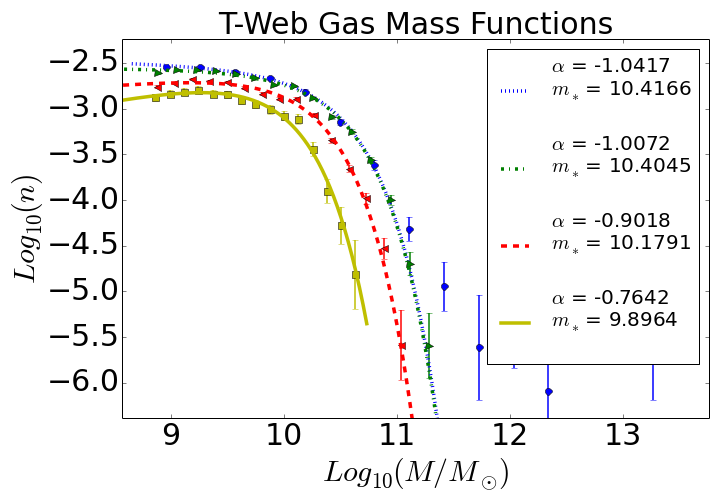
\includegraphics[width=0.5\textwidth]{environment2}
\label{fig2}
\caption{Mass functions with the environment defined from the Tidal
  Tensor web classification method.}
\centering
\end{figure}

 Taking into account the uncertainty on the the Schechter parameters
 we find  that the environment has an impact on the knee-mass,
 while for the faint-end slope we cannot find any change.
 This result is in agreement with the observational study by
\citealp{Jones}.


\begin{thebibliography}
\bibitem[Jones et al. 2016]{Jones} M. G. Jones, E. Papastergis, M. P. Haynes, and R. Giovanelli. Environmental dependence of the H I mass function in the ALFALFA 70\% catalogue. MNRAS, 457:4393–4405, April 2016.
\bibitem[Forero-Romero et al. 2009]{Forero} J. E. Forero-Romero, Y. Hoffman, S. Gottloeber, A. Klypin, and G. Yepes. A dynamical classification of the cosmic web. MNRAS, 396:1815–1824, July 2009.
\bibitem[Vogelsberger et al. 2014]{Vogelsberger}Vogelsberger, M., {Genel}, S.,
  {Springel}, V., {Torrey}, P.,  {Sijacki}, D., {Xu}, D.,
  {Snyder}, G., {Nelson}, D., {Hernquist}, L.. Introducing the
  Illustris Project: simulating the coevolution of dark and visible
  matter in the Universe. MNRAS, 444:1518-1547, October 2014.
\end{thebibliography}

\end{document}
